\chapter{Introduction}
\textit{Enseigné par Raphaël Dando}

\section{Contexte de Marché et Notation}

\subsection{Marché de la dette}

Le marché de la dette se divise en plusieurs segments principaux :
\begin{itemize}
    \item \textbf{Government bonds} : Obligations d'État.
    \item \textbf{Corporate bonds} : Obligations d'entreprises (notre focus principal).
    \item \textbf{Municipal bonds} : Obligations municipales.
    \item \textbf{Mortgage backed securities} : Titres adossés à des créances hypothécaires.
\end{itemize}

\subsection{Agences de notation et Ratings}

Les trois agences de notation principales sont : \textbf{S\&P}, \textbf{Moody's} et \textbf{Fitch}. Elles évaluent la solvabilité des émetteurs.

\subsubsection{Échelles de notation}

On distingue deux grandes catégories de notation :
\begin{itemize}
    \item \textbf{Investment Grade (IG)} : De AAA à BBB- (S\&P) ou Aaa à Baa3 (Moody's).
    \item \textbf{Speculative Grade (HY - High Yield)} : De BB+ à D (S\&P) ou Ba1 à C (Moody's).
\end{itemize}

\subsection{Transition de Rating}

Il est également crucial d'étudier les probabilités de transition de rating (par exemple, la probabilité qu'une obligation notée A passe à BBB en un an). C'est ce qu'on appelle la \textbf{matrice de transition}.

\begin{table}[H]
    \centering
    \begin{tabular}{|l|c|c|c|c|}
        \hline
        Rating initial & A & BBB & BB & Défaut \\ \hline
        A   & 90\% & 7\% & 2,9\% & 0,1\% \\ \hline
        BBB & ... & ... & ... & ... \\ \hline
        BB  & ... & ... & ... & ... \\ \hline
    \end{tabular}
    \caption{Exemple simplifié d'une matrice de transition (1 an)}
\end{table}

\subsection{Dynamique IG vs HY}

On observe des comportements différents selon la qualité de crédit :
\begin{itemize}
    \item \textbf{Investment Grade (IG)} : La courbe des PD tend à être \textbf{convexe}.
    \item \textbf{High Yield (HY)} : La courbe des PD tend à être \textbf{concave}.
\end{itemize}

\begin{figure}[H]
    \centering
    \begin{subfigure}{0.48\textwidth}
        \centering
        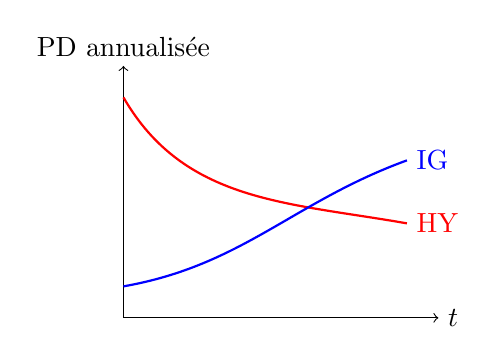
\begin{tikzpicture}[scale=0.8]
            % Axes
            \draw[->] (0,0) -- (5,0) node[right] {$t$};
            \draw[->] (0,0) -- (0,4) node[above] {PD annualisée};
            % HY curve (decreasing/concave)
            \draw[thick, red] (0,3.5) to[out=-60, in=170] (4.5,1.5);
            \node[red, right] at (4.5,1.5) {HY};
            % IG curve (increasing/convex)
            \draw[thick, blue] (0,0.5) to[out=10, in=-160] (4.5,2.5);
            \node[blue, right] at (4.5,2.5) {IG};
        \end{tikzpicture}
        \caption{Dynamique de la PD annualisée}
    \end{subfigure}
    \hfill
    \begin{subfigure}{0.48\textwidth}
        \centering
        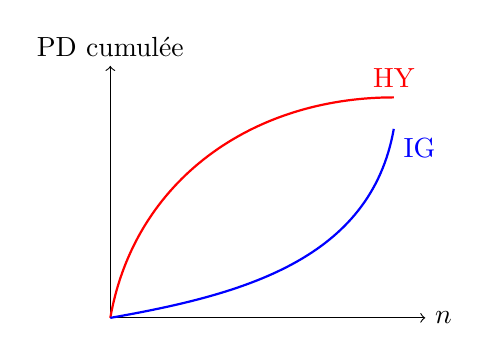
\begin{tikzpicture}[scale=0.8]
            % Axes
            \draw[->] (0,0) -- (5,0) node[right] {$n$};
            \draw[->] (0,0) -- (0,4) node[above] {PD cumulée};
            % HY curve (concave)
            \draw[thick, red] (0,0) to[out=80, in=180] (4.5,3.5);
            \node[red, above] at (4.5,3.5) {HY};
            % IG curve (convex)
            \draw[thick, blue] (0,0) to[out=10, in=-100] (4.5,3);
            \node[blue, below right] at (4.5,3) {IG};
        \end{tikzpicture}
        \caption{Dynamique de la PD cumulative}
    \end{subfigure}
    \caption{Évolution des probabilités de défaut selon le segment de crédit}
\end{figure}

\section{Fondamentaux du Risque de Crédit}

\subsection{Probabilité de Défaut (PD)}

À chaque rating est associée une probabilité de défaut. On distingue la probabilité de défaut annuelle et la probabilité de défaut cumulative.

\subsubsection{Relation entre PD annualisée et cumulative}

La probabilité de ne pas faire défaut jusqu'à l'année $n$ est le produit des probabilités de ne pas faire défaut chaque année $i$.
Soit $PD_{annualise}(i)$ la probabilité de défaut lors de l'année $i$ sachant qu'il n'y a pas eu de défaut avant.
La probabilité cumulative de défaut à l'horizon $n$, notée $PD_{cumul}(n)$, vérifie :
\begin{equation}
    1 - PD_{cumul}(n) = \prod_{i=1}^n \left( 1 - PD_{annualise}(i) \right)
\end{equation}

\subsection{Spreads et Recouvrement}

\begin{itemize}
    \item \textbf{Spreads annualisés} : Écart de taux par rapport à un taux sans risque, exprimé annuellement.
    \item \textbf{Taux de recouvrement (Recovery Rate - $R$)} : Pourcentage de la valeur nominale que l'investisseur récupère en cas de défaut.
    \item \textbf{Loss Given Default (LGD)} : La perte subie en cas de défaut, définie par $LGD = 1 - R$.
\end{itemize}

\subsection{Séniorité de la dette}

La position d'une créance dans la structure de capital d'une entreprise détermine son rang de priorité en cas de liquidation. Plus la dette est senior, plus le taux de recouvrement est élevé.

\begin{itemize}
    \item \textbf{Secured} (Dette sécurisée) : Garantie par des actifs spécifiques.
    \item \textbf{Senior Secured} : Priorité maximale parmi les dettes non garanties.
    \item \textbf{Senior Unsecured} : Taux de recouvrement historique moyen d'environ \textbf{40\%}.
    \item \textbf{Subordinated} (Dette subordonnée) : Payée après la dette senior.
    \item \textbf{Junior} : Priorité la plus basse, avec un taux de recouvrement souvent proche de \textbf{0\%}.
\end{itemize}

\subsection{Modélisation du taux de recouvrement}

Le taux de recouvrement $R$ est une variable aléatoire comprise entre 0 et 1. Il est fréquemment modélisé par une \textbf{loi Beta}, qui est très flexible et peut prendre différentes formes selon ses paramètres $\alpha$ et $\beta$ :
\begin{itemize}
    \item \textbf{Forme en U} (Bimodale, $\alpha < 1, \beta < 1$) : Cas fréquent pour le recouvrement, où l'on récupère soit très peu (proche de 0), soit la majeure partie (proche de 1).
    \item \textbf{Forme en cloche} (Unimodale, $\alpha > 1, \beta > 1$) : Cas où le recouvrement est concentré autour d'une valeur moyenne (ex: 40\%), ressemblant à une loi Normale.
\end{itemize}

\begin{figure}[H]
    \centering
    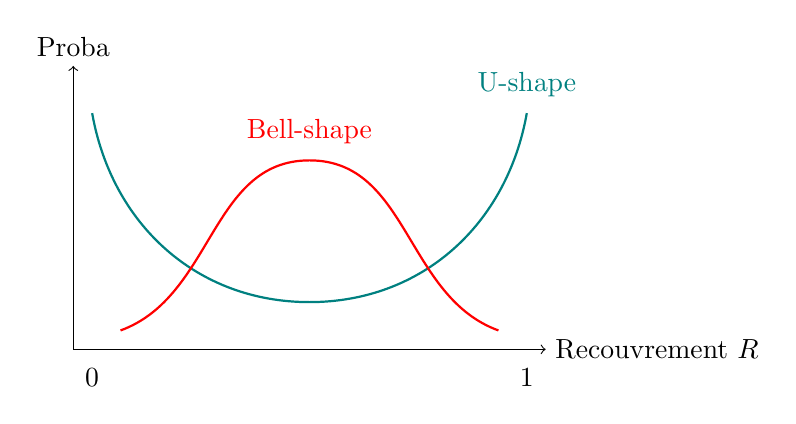
\begin{tikzpicture}[scale=1.2]
        % Axes
        \draw[->] (0,0) -- (5,0) node[right] {Recouvrement $R$};
        \draw[->] (0,0) -- (0,3) node[above] {Proba};
        
        % Beta distribution (U-shape) - Teal
        \draw[thick, teal] (0.2,2.5) to[out=-80, in=180] (2.5,0.5) to[out=0, in=-100] (4.8,2.5);
        \node[teal] at (4.8, 2.8) {U-shape};
        
        % Beta distribution (Bell-shape) - Red
        \draw[thick, red] (0.5,0.2) to[out=20, in=180] (2.5,2.0) to[out=0, in=160] (4.5,0.2);
        \node[red] at (2.5, 2.3) {Bell-shape};
        
        % Labels axes
        \node at (0.2,-0.3) {$0$};
        \node at (4.8,-0.3) {$1$};
    \end{tikzpicture}
    \caption{Flexibilité de la loi Beta pour modéliser le recouvrement}
\end{figure}

\subsection{Limites et Contexte Historique}

La gestion des risques de crédit a été fortement remise en question lors de la dernière crise financière (2008). 

\begin{itemize}
    \item \textbf{Paramètres fixes vs dynamiques} : Historiquement, les taux de recouvrement étaient souvent considérés comme fixes dans les modèles. En réalité, ils varient fortement avec le cycle économique (corrélation entre PD et LGD).
    \item \textbf{Erreurs de notation} : Les ratings sur les tranches seniors ont souvent été surévalués, car les modèles sous-estimaient la corrélation par les défauts et la variabilité des taux de recouvrement.
    \item \textbf{Impact systémique} : Une mauvaise évaluation de ces risques peut conduire à une sous-estimation massive du capital nécessaire pour couvrir les pertes.
\end{itemize}

Des changements de régime peuvent survenir selon les conditions de marché.

\section{Valorisation Standard et Mesures de Spread}

\subsection{Valorisation des Obligations (Bond Pricing)}

Avant de pricer une obligation, il est important de distinguer deux notions de prix :
\begin{itemize}
    \item \textbf{Clean Price} : Le prix coté sur les marchés, hors intérêts courus.
    \item \textbf{Dirty Price} : Le prix réellement payé lors de la transaction. Il inclut les \textbf{intérêts courus} (accrued interest) depuis le dernier détachement de coupon.
    \begin{equation}
        \text{Dirty Price} = \text{Clean Price} + \text{Accrued Interest}
    \end{equation}
\end{itemize}

\subsubsection{Modèle Discret des Flux}

Le prix d'une obligation à l'instant $t_0$ correspond à la somme de ses flux futurs actualisés (Coupons $C$ et Nominal $F$ à maturité $t_n$), en utilisant un taux de rendement (yield) $y$ :

\begin{equation}
    P(t_0) = \sum_{i=1}^n \frac{C}{(1+y)^{t_i - t_0}} + \frac{F}{(1+y)^{t_n - t_0}}
\end{equation}

\subsection{Spreads et Quantification du Risque}

Pour isoler et quantifier le risque de crédit, on compare le rendement de l'obligation à un taux sans risque ("Risk-Free Rate").

\subsubsection{Estimation de la courbe sans risque (Bootstrapping)}

Les taux sans risque $R_i$ pour différentes maturités ne sont pas toujours directement observables. On utilise la méthode de \textbf{Bootstrap} pour reconstituer la courbe des taux zéro-coupon (Zero-Coupon Yield Curve) de proche en proche à partir d'instruments liquides du marché (obligations d'État, swaps).

\subsubsection{Le Z-Spread (Zero-volatility Spread)}

Le \textbf{Z-Spread} (noté $Z$) est le spread constant qu'il faut ajouter à l'ensemble de la courbe des taux sans risque $R_i$ pour retrouver le prix de marché actuel de l'obligation.

\begin{equation}
    P_{\text{market}}(t_0) = \sum_{i=1}^n \frac{C}{(1 + R_i + Z)^{t_i - t_0}} + \frac{F}{(1 + R_i + Z)^{t_n - t_0}}
\end{equation}

\textbf{Interprétation :}
\begin{itemize}
    \item $Z$ capture principalement le \textbf{risque de crédit} de l'émetteur (et une prime de liquidité).
    \item Plus $Z$ est élevé, plus le prix de l'obligation est faible (pour une courbe sans risque donnée).
    \item Il permet de séparer le \textbf{risque de taux} (contenu dans $R_i$) du risque de crédit.
\end{itemize}

\subsubsection{Autres mesures de Spread}

\begin{itemize}
    \item \textbf{OAS (Option Adjusted Spread)} : Utilisé pour les obligations comportant des options cachées (ex: \textit{callable bonds}). L'OAS retire le prix de ces options pour donner un spread "pur", comparable à une obligation standard.
    \item \textbf{Asset Swap Spread (ASW)} : Spread obtenu lors d'un échange (Swap) où l'investisseur paie le coupon fixe de l'obligation et reçoit un taux variable (ex: Euribor) + Spread.
\end{itemize}

\section{Modélisation par Intensité de Défaut}

\subsection{Cadre d'Intensité de Défaut}

\subsubsection{Condition au Pair (Par Condition)}

Un résultat fondamental pour les obligations est la relation entre le taux de coupon et le rendement (yield) :
\begin{itemize}
    \item Si \textbf{Coupon = Yield}, alors le prix de l'obligation est égal à son nominal (100\%). On dit qu'elle cote au \textbf{Pair} (Par).
    \item Si Coupon $>$ Yield, elle cote au-dessus du Pair (Premium).
    \item Si Coupon $<$ Yield, elle cote en-dessous du Pair (Discount).
\end{itemize}

\subsubsection{Valorisation en Temps Continu}

Pour simplifier les modèles, on passe souvent en temps continu. Le prix d'une obligation sans risque payant un coupon continu $c$ jusqu'à maturité $T$ est donné par :
\begin{equation}
    P(t, T, c, r) = \int_t^T c e^{-r(u-t)} du + 1 \cdot e^{-r(T-t)}
\end{equation}
Ce qui se simplifie en :
\begin{equation}
    P = \frac{c}{r} (1 - e^{-r(T-t)}) + e^{-r(T-t)}
\end{equation}
On retrouve bien que si $c=r$, alors $P=1$.

\subsubsection{Probabilité de Survie et Intensité de Défaut}

On modélise l'instant de défaut $\tau$ comme le premier saut d'un processus de Poisson d'intensité $\lambda$ (hazard rate).
La probabilité de faire défaut dans un intervalle infinitésimal $dt$, sachant qu'on a survécu jusqu'à $t$, est :
\begin{equation}
    P(\tau \le t + dt \mid \tau > t) = \lambda dt
\end{equation}

La probabilité de survie $S(t)$ à l'instant $t$ (c'est-à-dire $P(\tau > t)$) suit alors une décroissance exponentielle :
\begin{equation}
    S(t) = e^{-\lambda t} \quad \text{(si } \lambda \text{ constant)}
\end{equation}

\begin{figure}[H]
    \centering
    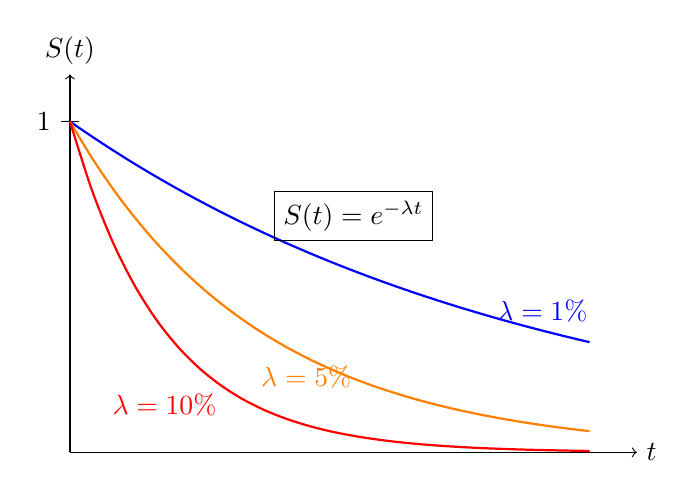
\begin{tikzpicture}[scale=1.2]
        % Axes
        \draw[->] (0,0) -- (6,0) node[right] {$t$};
        \draw[->] (0,0) -- (0,4) node[above] {$S(t)$};
        
        % S(0) = 1
        \draw (0.1,3.5) -- (-0.1,3.5) node[left] {$1$};
        
        % Curves for different lambdas
        \draw[thick, blue, domain=0:5.5, smooth, variable=\x] plot ({\x}, {3.5*exp(-0.2*\x)});
        \node[blue] at (5, 1.5) {$\lambda = 1\%$};
        
        \draw[thick, orange, domain=0:5.5, smooth, variable=\x] plot ({\x}, {3.5*exp(-0.5*\x)});
        \node[orange] at (2.5, 0.8) {$\lambda = 5\%$};
        
        \draw[thick, red, domain=0:5.5, smooth, variable=\x] plot ({\x}, {3.5*exp(-1.0*\x)});
        \node[red] at (1, 0.5) {$\lambda = 10\%$};
        
        % Equation box
        \node[draw, align=center] at (3, 2.5) {$S(t) = e^{-\lambda t}$};
        
    \end{tikzpicture}
    \caption{Probabilité de survie en fonction de l'intensité de défaut $\lambda$}
\end{figure}

\subsection{Valorisation d'une Obligation Risquée}

\subsubsection{Cas Zero Recovery}

Considérons une obligation risquée payant un coupon continu $c$ jusqu'à maturité $T$, mais avec un \textbf{taux de recouvrement nul} ($R=0$).
Cela signifie que si le défaut survient à $\tau \le T$, tous les paiements futurs (coupons et nominal) sont perdus.

\begin{figure}[H]
    \centering
    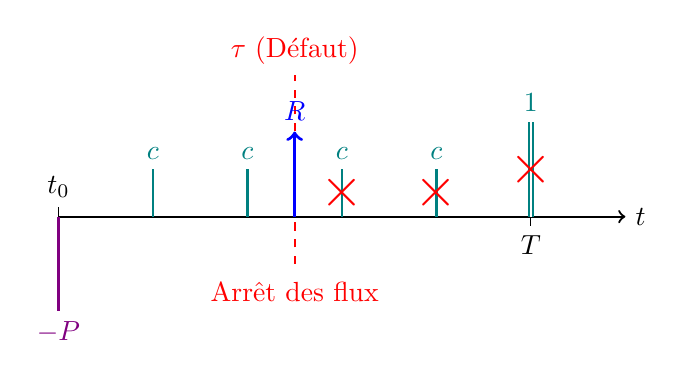
\begin{tikzpicture}[scale=1.2]
        % Timeline
        \draw[->, thick] (0,0) -- (6,0) node[right] {$t$};
        
        % T_0 and T
        \draw (0,0.1) -- (0,-0.1);
        \node[above] at (0, 0.1) {$t_0$};
        \draw (5,0.1) -- (5,-0.1) node[below] {$T$};
        
        % Initial Price -P
        \draw[thick, violet] (0, 0) -- (0, -1) node[below] {$-P$};

        % Coupons
        \foreach \x in {1,2,3,4}
            \draw[teal, thick] (\x, 0) -- (\x, 0.5) node[above] {$c$};
            
        % Nominal
        \draw[teal, thick, double] (5, 0) -- (5, 1) node[above] {$1$};
        
        % Default event
        \draw[red, thick, dashed] (2.5, -0.5) -- (2.5, 1.5) node[above] {$\tau$ (Défaut)};
        
        % Recovery Flow
        \draw[blue, very thick, ->] (2.5, 0) -- (2.5, 0.9) node[above] {$R$};

        \node[red, align=center] at (2.5, -0.8) {Arrêt des flux};
        
        % Cross out future flows (3, 4, 5)
        \node[red, scale=2] at (3, 0.25) {$\times$};
        \node[red, scale=2] at (4, 0.25) {$\times$};
        \node[red, scale=2] at (5, 0.5) {$\times$};
        
    \end{tikzpicture}
    \caption{Scénario de défaut : Perte des flux futurs}
\end{figure}

Le prix de l'obligation est l'espérance des flux futurs actualisés, conditionnée par la survie jusqu'à la maturité des flux :

\begin{equation}
    P(t, T) = \mathbb{E} \left[ \int_t^T c e^{-r(u-t)} \mathbb{1}_{\tau > u} du + e^{-r(T-t)} \mathbb{1}_{\tau > T} \right]
\end{equation}

En utilisant l'indépendance entre le taux sans risque $r$ et le temps de défaut $\tau$, et sachant que $\mathbb{E}[\mathbb{1}_{\tau > u}] = P(\tau > u) = e^{-\lambda(u-t)}$, on obtient :

\begin{equation}
    P(t, T) = \int_t^T c e^{-(r+\lambda)(u-t)} du + e^{-(r+\lambda)(T-t)}
\end{equation}

En résolvant l'intégrale :
\begin{equation}
    P(t, T) = \frac{c}{r+\lambda} (1 - e^{-(r+\lambda)(T-t)}) + e^{-(r+\lambda)(T-t)}
\end{equation}
Ou encore, sous une forme faisant apparaître l'écart au pair :
\begin{equation}
    P(t, T) = 1 + (c - r - \lambda) \frac{1 - e^{-(r+\lambda)(T-t)}}{r+\lambda}
\end{equation}

\textbf{Conclusion importante :}
Dans ce modèle avec recouvrement nul, on actualise les flux au taux $r + \lambda$.
Par identification avec la formule du Z-Spread ($P$ actualisé à $r + Z$), on a donc :
\begin{tcolorbox}[colback=red!5!white,colframe=red!75!black,title=Relation Intensité - Spread]
    Si le taux de recouvrement est nul ($R=0$), alors le spread de crédit est égal à l'intensité de défaut :
    \begin{equation}
        Z = \lambda
    \end{equation}
\end{tcolorbox}

\subsubsection{Cas Général avec Recouvrement ($R \neq 0$)}

Si l'on suppose maintenant qu'en cas de défaut à l'instant $\tau$, l'investisseur récupère une fraction $R$ du nominal (ou de la valeur de marché, selon la convention).
Le prix de l'obligation devient la somme de deux termes :
\begin{itemize}
    \item La valeur des flux promis tant qu'il n'y a pas de défaut (partie "Zero Recovery").
    \item La valeur présente du paiement de recouvrement au moment du défaut.
\end{itemize}

\begin{equation}
    P(t, T) = \underbrace{\int_t^T c e^{-(r+\lambda)(u-t)} du + e^{-(r+\lambda)(T-t)}}_{\text{Zero Recovery Price}} + \underbrace{\mathbb{E} \left[ e^{-r(\tau-t)} R \cdot \mathbb{1}_{\tau \le T} \right]}_{\text{Recovery Part}}
\end{equation}

Le terme de recouvrement se calcule en intégrant sur la densité de défaut $f(\tau) = \lambda e^{-\lambda(\tau-t)}$ :
\begin{equation}
    \text{Recovery Part} = \int_t^T e^{-r(u-t)} R \cdot \lambda e^{-\lambda(u-t)} du = R \lambda \int_t^T e^{-(r+\lambda)(u-t)} du
\end{equation}

En regroupant les termes, on obtient une formule élégante mettant en jeu la perte attendue $(1-R)\lambda$ :

\begin{equation}
    P(t, T) = 1 + (c - r - (1-R)\lambda) \times \frac{1 - e^{-(r+\lambda)(T-t)}}{r+\lambda}
\end{equation}

\begin{tcolorbox}[colback=blue!5!white,colframe=blue!75!black,title=Approximation du Spread]
    En comparant avec la formule du Z-Spread, on en déduit que le spread de crédit $Z$ est approximativement égal au produit de la perte en cas de défaut (LGD) et de l'intensité de défaut :
    \begin{equation}
        Z \approx (1-R)\lambda = \text{LGD} \times \text{PD intensity}
    \end{equation}
\end{tcolorbox}

\subsubsection{Durée Risquée et Spread de Crédit}

Pour formaliser cette relation, on introduit la notion de **Risky Duration** (Durée Risquée), qui correspond à la valeur présente d'une unité monétaire reçue en continu jusqu'au minimum de $T$ et $\tau$ :

\begin{equation}
    \text{Risky Duration} = \int_t^T e^{-(r+\lambda)(u-t)} du = \frac{1 - e^{-(r+\lambda)(T-t)}}{r+\lambda}
\end{equation}

On peut alors réécrire le prix de l'obligation risquée (avec recouvrement $R$) de manière très intuitive :

\begin{equation}
    P(t, T) = 1 + (c - r - S) \times \text{Risky Duration}
\end{equation}

Où $S$ est le **Credit Spread** défini par :
\begin{equation}
    S = (1-R)\lambda
\end{equation}

Cela montre que l'écart de prix par rapport au pair ($P-1$) est proportionnel à la différence entre le coupon $c$ et le coût total du risque ($r+S$), multipliée par la durée d'exposition au risque.

Enfin, pour des temps courts ($t$ petit), on a l'approximation suivante pour la probabilité de défaut cumulée :
\begin{equation}
    P(\tau \le t) = 1 - e^{-\lambda t} \approx \lambda t
\end{equation}

\subsection{Credit Default Swaps (CDS)}

\subsubsection{Définition et Mécanisme}

Le \textbf{Credit Default Swap (CDS)} est un instrument financier dérivé qui permet de transférer le risque de crédit d'une entité de référence d'une contrepartie à une autre. C'est essentiellement un contrat d'assurance contre le défaut.

Dans un contrat CDS :
\begin{itemize}
    \item L'\textbf{Acheteur de Protection} (Protection Buyer) verse une prime périodique (le spread CDS) au vendeur de protection.
    \item Le \textbf{Vendeur de Protection} (Protection Seller) s'engage à compenser l'acheteur en cas d'événement de crédit sur l'entité de référence.
\end{itemize}

\begin{figure}[H]
    \centering
    \begin{tikzpicture}[scale=1, transform shape]
        % Styles
        \tikzstyle{block} = [rectangle, draw, thick, text width=3cm, text centered, minimum height=2cm, rounded corners]
        \tikzstyle{arrow} = [thick, ->, >=stealth]
        
        % Nodes
        \node (buyer) [block, fill=blue!10] {\textbf{Protection Buyer}\\ (Acheteur)};
        \node (seller) [block, fill=green!10, right=7cm of buyer] {\textbf{Protection Seller}\\ (Vendeur)};
        
        % Arrows
        % Premium flow (Buyer -> Seller)
        \draw [arrow, teal] (buyer.east) -- node[below, align=center] {Premium\\ (Spread / Flux périodique)} (seller.west);
        
        % Protection flow (Seller -> Buyer)
        \draw [arrow, red, dashed] ([yshift=0.5cm]seller.west) -- node[above, align=center] {Paiement si \textit{Credit Event}\\ $(1-R)$} ([yshift=0.5cm]buyer.east);
        
    \end{tikzpicture}
    \caption{Mécanisme des flux d'un CDS}
    \label{fig:cds_flows}
\end{figure}

Si aucun événement de crédit ne survient jusqu'à la maturité du contrat, le vendeur de protection conserve les primes reçues et ne paie rien. Si un défaut survient, le vendeur paie à l'acheteur la perte encourue (généralement le nominal moins le taux de recouvrement, soit $1-R$).

\subsubsection{Événements de Crédit (ISDA)}

Les événements déclenchant le paiement de la protection sont standardisés par l'\textbf{ISDA} (International Swaps and Derivatives Association). Les principaux sont :

\begin{enumerate}
    \item \textbf{Bankruptcy (Faillite)} : L'entité de référence est officiellement en faillite ou insolvable.
    \item \textbf{Failure to Pay (Défaut de Paiement)} : L'entité manque un paiement d'intérêts ou de principal sur sa dette (après une période de grâce).
    \item \textbf{Restructuring (Restructuration)} : Modification des termes de la dette (réduction du principal, baisse du coupon, allongement de la maturité) qui est défavorable aux créanciers.
\end{enumerate}

D'autres événements peuvent exister selon les contrats (e.g., \textit{Obligation Acceleration}, \textit{Repudiation/Moratorium}), mais les trois ci-dessus sont les plus standards pour les entreprises (Corporate CDS).

\subsubsection{Utilisation des CDS}

Les CDS sont utilisés pour plusieurs objectifs distincts :

\begin{itemize}
    \item \textbf{Hedging (Couverture)} :
    \begin{itemize}
        \item \textbf{Marché} : Se protéger contre une baisse de la valeur des obligations détenues (due à une hausse du risque de crédit).
        \item \textbf{Bilan (Regulatory Capital)} : "Alléger le bilan" en transférant le risque. Cela permet de réduire les exigences en capital réglementaire (Economic Capital Relief) sans vendre l'actif sous-jacent.
    \end{itemize}
    \item \textbf{Spéculation} : Parier sur la dégradation de la qualité de crédit d'une entité sans détenir sa dette (Naked CDS).
    \item \textbf{Levier} : S'exposer au risque de crédit avec un capital initial faible (le spread) par rapport au montant notionnel.
\end{itemize}

\subsubsection{Valorisation et Flux (Cash Flows)}

Un CDS est un échange de deux jambes de flux :

\textbf{1. Jambe Fixe (Fixed Leg) - Le Premium} \\
L'acheteur de protection paie le spread $S$ sur le montant nominal $N$ à des dates fixées $t_1, \dots, t_n$, tant que l'événement de crédit n'a pas eu lieu ($\tau > t_i$).
La valeur présente de cette jambe est (en approximation discrète) :
\begin{equation}
    \text{Fixed Leg} = \sum_{i=1}^n S \times N \times \Delta t_i \times \mathbb{E}[e^{-r t_i} \mathbb{1}_{\tau > t_i}] = S \cdot N \sum_{i=1}^n \Delta t_i e^{-r t_i} S(t_i)
\end{equation}

Une version continue (souvent utilisée pour les calculs théoriques) s'écrit :
\begin{equation}
    V_{\text{fixed}} = \mathbb{E} \left[ \int_{t_0}^T S e^{-r(u-t_0)} \mathbb{1}_{\tau > u} du \right] = S \times \text{Risky Duration}
\end{equation}

\textbf{2. Jambe Variable (Floating Leg) - La Protection} \\
Le vendeur de protection paie la perte $(1-R)$ sur le nominal $N$ si le défaut survient avant la maturité ($\tau \le T$).
Ce paiement se fait généralement peu de temps après le défaut $\tau$.
\begin{equation}
    \text{Floating Leg} = \mathbb{E} \left[ e^{-r \tau} (1-R) \times N \times \mathbb{1}_{\tau \le T} \right]
\end{equation}

En temps continu, avec une intensité de défaut $\lambda$ consante, on peut expliciter ce calcul :
\begin{align}
    \text{Floating Leg} &= \int_{t_0}^T (1-R) N e^{-r(u-t_0)} \underbrace{\lambda e^{-\lambda(u-t_0)}}_{\text{densité de } \tau} du \\
    &= (1-R) N \lambda \int_{t_0}^T e^{-(r+\lambda)(u-t_0)} du \\
    &= (1-R) N \lambda \times \text{Risky Duration} \\
    &= (1-R) N \frac{\lambda}{r+\lambda} (1 - e^{-(r+\lambda)(T-t_0)})
\end{align}

\begin{figure}[H]
    \centering
    \begin{subfigure}{\textwidth}
        \centering
        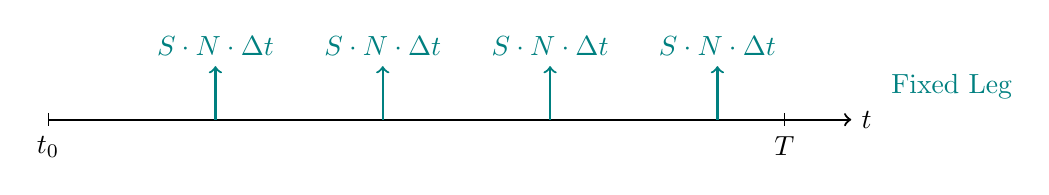
\begin{tikzpicture}[scale=0.85]
            % Timeline Fixed Leg
            \draw[->, thick] (0,0) -- (12,0) node[right] {$t$};
            \draw (0,0.1) -- (0,-0.1) node[below] {$t_0$};
            \draw (11,0.1) -- (11,-0.1) node[below] {$T$};
            
            % Payments - WIDENED SPACING
            \foreach \x in {2.5, 5, 7.5, 10}
                \draw[teal, thick, ->] (\x, 0) -- (\x, 0.8) node[above] {$S \cdot N \cdot \Delta t$};
            
            \node[teal, align=center] at (13.5, 0.5) {Fixed Leg};
        \end{tikzpicture}
        \caption{Fixed Leg : Paiement du Premium}
    \end{subfigure}
    
    \vspace{0.5cm}
    
    \begin{subfigure}{\textwidth}
        \centering
        \begin{tikzpicture}[scale=0.85]
            % Timeline Floating Leg
            \draw[->, thick] (0,0) -- (12,0) node[right] {$t$};
            \draw (0,0.1) -- (0,-0.1) node[below] {$t_0$};
            \draw (11,0.1) -- (11,-0.1) node[below] {$T$};
            
            % Default time tau
            \draw[red, dashed] (6, -0.5) -- (6, 1.5) node[above] {$\tau$};
            
            % Payment at tau
            \draw[red, very thick, ->] (6, 0) -- (6, 1.2) node[above, xshift=1.5cm] {$(1-R) \cdot N$};
            
            \node[red, align=center] at (13.5, 0.5) {Floating Leg};
        \end{tikzpicture}
        \caption{Floating Leg : Paiement de la Protection}
    \end{subfigure}
    \caption{Flux de trésorerie d'un CDS}
\end{figure}


\subsubsection{Spread de CDS Équitable (Fair Spread)}

À l'initiation du contrat, le spread $S$ est déterminé pour que la valeur nette du CDS soit nulle (absence d'arbitrage). On égalise la valeur des deux jambes :

\begin{equation}
    \text{Fixed Leg} = \text{Floating Leg}
\end{equation}

En utilisant les formules continues dérivées ci-dessus :
\begin{equation}
    S \times N \times \text{Risky Duration} = (1-R) \times N \times \lambda \times \text{Risky Duration}
\end{equation}

En simplifiant par $N$ et par la Risky Duration (supposée non nulle), on obtient la relation fondamentale liant le spread de CDS à l'intensité de défaut et au taux de recouvrement :

\begin{tcolorbox}[colback=blue!5,colframe=blue!40,title=Formule du Spread de CDS (Fair Value)]
\begin{equation}
    S = (1-R) \lambda
\end{equation}
\end{tcolorbox}

Cette relation est très intuitive : le coût de la protection ($S$) est égal à la perte attendue par unité de temps ($\lambda \times (1-R)$).
\begin{itemize}
    \item Si le risque de défaut $\lambda$ augmente, le spread $S$ augmente.
    \item Si le taux de recouvrement $R$ augmente, la perte potentielle diminue, donc le spread $S$ diminue.
\end{itemize}

\textbf{Market Value en cours de vie} \\
Si les conditions de marché changent (ex: le spread de marché devient $S_{\text{new}}$), la valeur pour l'acheteur d'un CDS signé à $S_{\text{old}}$ est approximativement :
\begin{equation}
    V_{\text{buyer}} \approx (S_{\text{new}} - S_{\text{old}}) \times \text{Risky Duration} \times N
\end{equation}
Cela montre que l'acheteur gagne si le spread s'écarte (le crédit se détériore).
